
%
% The first command in your LaTeX source must be the \documentclass command.
\documentclass[acmlarge,screen]{acmart}

\usepackage[T1,T2A]{fontenc}
\usepackage[utf8]{inputenc}
\usepackage[english,russian]{babel}
% \usepackage{epstopdf,cmap,amsfonts,amsmath,mathtext,enumerate,float,natbib,indentfirst,hyperref,graphicx,multirow,setspace}
% \usepackage{newtxtext,newtxmath}
% pscyr used for good quality russian font rendering. See http://blog.harrix.org/?p=444 for the full installing instruction of pscyr. 
% \usepackage{pscyr}


%
% defining the \BibTeX command - from Oren Patashnik's original BibTeX documentation.
\def\BibTeX{{\rm B\kern-.05em{\sc i\kern-.025em b}\kern-.08emT\kern-.1667em\lower.7ex\hbox{E}\kern-.125emX}}


% \usepackage[cm-default]{fontspec} % or install lmodern
% \usepackage{xltxtra} % load xunicode
% \usepackage[russian]{babel}
% \usepackage{xecyr}

% Rights management information. 
% This information is sent to you when you complete the rights form.
% These commands have SAMPLE values in them; it is your responsibility as an author to replace
% the commands and values with those provided to you when you complete the rights form.
%
% These commands are for a PROCEEDINGS abstract or paper.
\copyrightyear{2021}
\acmYear{2021}
\setcopyright{acmlicensed}
\acmConference[Woodstock '21]{Woodstock '21: ACM Symposium on Neural Gaze Detection}{June 03--05, 2018}{Woodstock, NY}
\acmBooktitle{Woodstock '21: ACM Symposium on Neural Gaze Detection, June 03--05, 2018, Woodstock, NY}
\acmPrice{15.00}
\acmDOI{10.1145/1122445.1122456}
\acmISBN{978-1-4503-9999-9/18/06}

%
% These commands are for a JOURNAL article.
%\setcopyright{acmcopyright}
%\acmJournal{TOG}
%\acmYear{2018}\acmVolume{37}\acmNumber{4}\acmArticle{111}\acmMonth{8}
%\acmDOI{10.1145/1122445.1122456}

%
% Submission ID. 
% Use this when submitting an article to a sponsored event. You'll receive a unique submission ID from the organizers
% of the event, and this ID should be used as the parameter to this command.
%\acmSubmissionID{123-A56-BU3}

%
% The majority of ACM publications use numbered citations and references. If you are preparing content for an event
% sponsored by ACM SIGGRAPH, you must use the "author year" style of citations and references. Uncommenting
% the next command will enable that style.
%\citestyle{acmauthoryear}

%
% end of the preamble, start of the body of the document source.
\begin{document}

%
% The "title" command has an optional parameter, allowing the author to define a "short title" to be used in page headers.
\title{Блокчейн-платформа hschain и язык смартконтрактов}

%
% The "author" command and its associated commands are used to define the authors and their affiliations.
% Of note is the shared affiliation of the first two authors, and the "authornote" and "authornotemark" commands
% used to denote shared contribution to the research.
\author{Сергей Зефиров}
\affiliation{%
  \institution{HEX Research}
  \city{Москва}
  \country{Россия}}
\email{larst@affiliation.org}

\author{Алексей Худяков}
\affiliation{%
  \institution{HEX Research}
  \city{Королёв}
  \country{Россия}}
\email{larst@affiliation.org}

\author{Антон Холомьёв}
\affiliation{%
  \institution{HEX Research}
  \city{Подольск}
  \country{Россия}
}


%
% By default, the full list of authors will be used in the page headers. Often, this list is too long, and will overlap
% other information printed in the page headers. This command allows the author to define a more concise list
% of authors' names for this purpose.
\renewcommand{\shortauthors}{Trovato and Tobin, et al.}

%
% The abstract is a short summary of the work to be presented in the article.
\begin{abstract}
В статье представлен обзор платформы для реализации блокчейн-приложений hschain и языка
смартконтрактов hschain-utxo. Платформа hschain позволяет создавать блокчейн приложения
на языке Haskell в виде конечных автоматов, правила валидации транзакций
являются переходами состояний и в отличие от многих решений не фиксированы,
а являются интерфейсом. Этот гибкий подход даёт возможность построения различных систем
основанных на технологии блокчейн.
\end{abstract}

%
% The code below is generated by the tool at http://dl.acm.org/ccs.cfm.
% Please copy and paste the code instead of the example below.
%
\begin{CCSXML}
<ccs2012>
 <concept>
  <concept_id>10010520.10010553.10010562</concept_id>
  <concept_desc>Computer systems organization~Embedded systems</concept_desc>
  <concept_significance>500</concept_significance>
 </concept>
 <concept>
  <concept_id>10010520.10010575.10010755</concept_id>
  <concept_desc>Computer systems organization~Redundancy</concept_desc>
  <concept_significance>300</concept_significance>
 </concept>
 <concept>
  <concept_id>10010520.10010553.10010554</concept_id>
  <concept_desc>Computer systems organization~Robotics</concept_desc>
  <concept_significance>100</concept_significance>
 </concept>
 <concept>
  <concept_id>10003033.10003083.10003095</concept_id>
  <concept_desc>Networks~Network reliability</concept_desc>
  <concept_significance>100</concept_significance>
 </concept>
</ccs2012>
\end{CCSXML}

\ccsdesc{proof of work}
\ccsdesc{Smartcontracts}
\ccsdesc{Blockchain}

%
% Keywords. The author(s) should pick words that accurately describe the work being
% presented. Separate the keywords with commas.
\keywords{blockchain, network, smartcontracts, proof of work}

%
% A "teaser" image appears between the author and affiliation information and the body 
% of the document, and typically spans the page. 
%%\begin{teaserfigure}
%%  \includegraphics[width=\textwidth]{sampleteaser}
%%  \caption{Seattle Mariners at Spring Training, 2010.}
%%  \Description{Enjoying the baseball game from the third-base seats. Ichiro Suzuki preparing to bat.}
%%  \label{fig:teaser}
%%\end{teaserfigure}

%
% This command processes the author and affiliation and title information and builds
% the first part of the formatted document.
\maketitle

\section{Сравнение подходов}

Практически все современные системы доказательства работы основаны на переборе с 
отсевом: Bitcoin, Etherium, Monero, Ergo и многие другие следуют по стопам HashCash 
(перебираем значения нескольких составляющих блока и отсеиваем путём сравнения криптосуммы 
заголовка блока с некоторым значением), а PrimeCoin перебирает простые числа определённого вида.

В любом случае, это задача перебора.

Классическая задача перебора, с которой началась теория сложности, это решение задачи выполнимости 
для некоторой логической формулы. При каких значениях входов некоторая логическая формула является выполнимой? 
Зная решение, очень просто проверить его через подстановку значений и вычисления по структуре формулы. 
Однако отыскать решение решительно сложно.

\section{Подробнее про логические задачи}

Один из вариантов логической формулы является коньюнктивная нормальная форма (КНФ или CNF по английски) - 
логическое И логических ИЛИ, состоящих из одного или более литерала (литерал это либо значение переменной, 
либо инверсия значения переменной).

Обычно, КНФ строят из описания какой-либо логической схемы или задачи, однако один из вариантов 
построения КНФ это случайная КНФ с дизъюнктами (логическими ИЛИ) из заданного количества литералов, 
которые выбираются случайными образом. Такие случайные КНФ не несут какого-либо смысла, тем не менее, они 1) 
так же сложны, как и КНФ для задач из практики, их решение отыскать так же сложно, 2) обычно, они имеют более, 
чем одно решение и 3) вероятность существования решения, сложность его отыскания и количество решений 
статистически определяются параметрами КНФ: количеством переменных, размером дизъюнкта и количеством дизъюнктов.

\section{Логическая задача, как часть фильтра для отсева блоков}

Что Bitcoin, что другие формируют заголовок блока и перебирают значения некоторых полей заголовка, 
чтобы получить криптосумму меньше, чем порог сложности. Обычно, это последнее поле заголовка - 
так называемый nonce (Number used Only oNCE), одноразовое число. Размер этого поля невелик, 
в районе 32-64 битов и никаких ограничений, кроме размера, на него не накладывается.

Мы предлагаем иметь большое одноразовое число, размером 256 битов, и наложить на него ограничение, 
что это поле содержит в себе решение для случайной КНФ с дизъюнктами из пяти литералов (от 256 переменных), 
состоящей из 5250 дизъюнктов. Случайная КНФ получается из криптосуммы части заголовка до одноразового числа. 
Криптосумма от полного заголовка блока (включая одноразовое число-решение) должна удовлетворять критерию сложности (быть меньше, чем порог сложности).

\section{Поиск решения, как ограничивающий фактор}

Многие современные системы доказательства работы (PoW) предпочитают полагаться на пропускную способность 
канала с внешней памятью, нежели на простое вычисление относительно простой функции (SHA256d в случае Bitcoin). 
Это относится к Ergo, Monero, Etherium и многим другим. Считается, что пропускная способность 
памяти масштабируется тяжелее, чем простые вычисления (что справедливо).

Однако уверенного размена достичь довольно сложно. Например, если использовать scrypt, 
который сперва заполняет память с помощью последовательного применения криптосуммы, 
а потом производит произвольную выборку из памяти по случайным адресам, 
то легко разменять пропускную способность памяти на вычислительные мощности 
(писать в память только, допустим, каждое восьмое значение, а семь оставшихся вычислять - что, 
как показывает практика ASIC для Bitcoin, легко достижимо и очень и очень энергоэффективно). 
Что Etherium, что Ergo, что Monero/RandomX имеют сходную структуру и позволяют либо перевычислять 
значения, либо склеивать выборки из памяти, уменьшая эффективную задержку.

Использование пропускной способности памяти можно обобщить до алгоритма, заметная часть которого 
последовательна и связана с поддержанием какого-то сравнительно большого состояния.

Современные алгоритмы решения задач булевой выполнимости как раз таковы - заметная доля их 
выполнения последовательна. Для полных алгоритмов решения надо поддерживать дизъюнкты в разного 
рода списках и статистику для определения очередной переменной для расщепления выбора. 
Для алгоритмов решения методом случайного поиска необходимо использовать и поддерживать 
актуальную статистику по переменным и дизъюнктам после изменения решения хотя бы на один бит.

Параметры задачи (5250 дизъюнктов из пяти литералов от 256 переменных на данный момент) таковы, что отыскание хоть какого-то решения занимает полсекунды на современном процессоре. Поиск последующих решений несколько быстрее - порядка 3-4 миллисекунд, - однако иногда алгоритм снова может потратить несколько сотен микросекунд на поиск. Поэтому среднее количество решений в секунду составляет, примерно, 30-50 решений, или, поскольку время на вычисление полной криптосуммы загадки пренебрежимо мало, 30-50 криптозагадок в секунду. Это сравнимо с довольно медленным Monero/RandomX с его ~200 ответов криптозагадок в секунду. Надо отметить, что здесь речь идёт не о полностью подходящих решениях (проходящих порог сложности), а всего лишь о каких-то кандидатах, некоторые из которых могут и подходить по сложности.

\section{Параллельное выполнение и ASIC}

Как ни странно, но на GPU современные методы решения задач булевой выполнимости укладываются 
довольно посредственно. Это связано с необходимостью поддержания своей копии 
статистики для каждого (частичного) решения, а эта статистика занимает довольно большой объём 
и находится в существенно далёких областях памяти. Поэтому: с одной стороны, всего 256 битов/переменных, 
с другой стороны 5250 ограничений, по разному связанных с этими битами. В сумме получается 128К 
на хранение статистики для решения и выше. Настолько большое расстояние, плюс одновременное 
выполнение команд на всех ядрах блока нитей GPU приводит к слабой утилизации вычислительных возможностей GPU.

Однако, 128 килобайт не так, чтобы и много для памяти около специализированного ядра в ASIC. Это, 
примерно, 12 квадратных миллиметров, по моим прикидкам. То есть, возможно получить довольно 
производительную систему с помощью программирования на Verilog/VHDL, если нам такое понадобится.

\section{Основные свойства}

При уменьшении порога вдвое время на поиск решения увеличивается, примерно, вдвое. Таким образом мы 
можем прогнозировать, как скажется изменение порога сложности на производительности PoW.

Фиксация части переменных для разбиения на подзадачи работает довольно плохо. Если мы знаем решение 
задачи и подаём на решатель задачц, в которой части этого решения уже зафиксирована (например, если есть решение с x0=Ложь, то мы создаём обычную задачу и добавляем дизхюнкт из одного литерала {!x0}), то решатель совершенно необязательно сможет отыскать решение, вроде бы, более простой задачи. Поэтому поиск решения лучше выполнять последовательно, для одного заголовка.

Поиск разных решений осуществляется добавлением ограничения, отсекающего текущее решение. Это, 
во-первых, увеличивает количество ограничений и время на их обработку и, во-вторых, всё более меняет 
структуру задачи. Если раньше она была случайной задачей из 5-литеральных дизъюнктов, то теперь 
среднее количество литералов увеличивается и эвристики перестают работать - увеличивая время поиска 
решения ещё больше.

\section{Заключение}

Мы предлагаем использовать решение случайной задачи булевой выполнимости, в качестве основной 
загадки для системы доказательства работы.

Это, с одной стороны, очень простая в формулировке задача, с другой стороны, её исследуют вот уже 50 лет 
с умеренным успехом и современное состояние дел не позволяет решать её очень быстро. А прогресс 
за последние десятилетия позволяет прогнозировать, что и в ближайшем будущем решение такого рода задач 
не будет ускорено сколько-нибудь сильно.

В настоящий момент у нас есть работающий код для предлагаемого варианта PoW. У нас, также, 
есть опыт создания решений для FPGA для похожих задач, поэтому мы сможем предложить 
сотрудничество для желающих создавать ASIC решения для нашей системы PoW.

\section{Sectioning Commands}

Your work should use standard \LaTeX\ sectioning commands: \verb|section|, \verb|subsection|, \verb|subsubsection|, and \verb|paragraph|. They should be numbered; do not remove the numbering from the commands. 

Simulating a sectioning command by setting the first word or words of a paragraph in boldface or italicized text is {\bf not allowed.}

\section{Tables}

The ``\verb|acmart|'' document class includes the ``\verb|booktabs|'' package --- \url{https://ctan.org/pkg/booktabs} --- for preparing high-quality tables. 

Table captions are placed {\it above} the table.

Because tables cannot be split across pages, the best placement for them is typically the top of the page nearest their initial cite.  To ensure this proper ``floating'' placement of tables, use the environment \textbf{table} to enclose the table's contents and the table caption.  The contents of the table itself must go in the \textbf{tabular} environment, to be aligned properly in rows and columns, with the desired horizontal and vertical rules.  Again, detailed instructions on \textbf{tabular} material are found in the \textit{\LaTeX\ User's Guide}.

Immediately following this sentence is the point at which Table~\ref{tab:freq} is included in the input file; compare the placement of the table here with the table in the printed output of this document.

\begin{table}
  \caption{Frequency of Special Characters}
  \label{tab:freq}
  \begin{tabular}{ccl}
    \toprule
    Non-English or Math&Frequency&Comments\\
    \midrule
    \O & 1 in 1,000& For Swedish names\\
    $\pi$ & 1 in 5& Common in math\\
    \$ & 4 in 5 & Used in business\\
    $\Psi^2_1$ & 1 in 40,000& Unexplained usage\\
  \bottomrule
\end{tabular}
\end{table}

To set a wider table, which takes up the whole width of the page's live area, use the environment \textbf{table*} to enclose the table's contents and the table caption.  As with a single-column table, this wide table will ``float'' to a location deemed more desirable. Immediately following this sentence is the point at which Table~\ref{tab:commands} is included in the input file; again, it is instructive to compare the placement of the table here with the table in the printed output of this document.

\begin{table*}
  \caption{Some Typical Commands}
  \label{tab:commands}
  \begin{tabular}{ccl}
    \toprule
    Command &A Number & Comments\\
    \midrule
    \texttt{{\char'134}author} & 100& Author \\
    \texttt{{\char'134}table}& 300 & For tables\\
    \texttt{{\char'134}table*}& 400& For wider tables\\
    \bottomrule
  \end{tabular}
\end{table*}

\section{Math Equations}
You may want to display math equations in three distinct styles:
inline, numbered or non-numbered display.  Each of
the three are discussed in the next sections.

\subsection{Inline (In-text) Equations}
A formula that appears in the running text is called an
inline or in-text formula.  It is produced by the
\textbf{math} environment, which can be
invoked with the usual \texttt{{\char'134}begin\,\ldots{\char'134}end}
construction or with the short form \texttt{\$\,\ldots\$}. You
can use any of the symbols and structures,
from $\alpha$ to $\omega$, available in
\LaTeX~\cite{Lamport:LaTeX}; this section will simply show a
few examples of in-text equations in context. Notice how
this equation:
\begin{math}
  \lim_{n\rightarrow \infty}x=0
\end{math},
set here in in-line math style, looks slightly different when
set in display style.  (See next section).

\subsection{Display Equations}
A numbered display equation---one set off by vertical space from the
text and centered horizontally---is produced by the \textbf{equation}
environment. An unnumbered display equation is produced by the
\textbf{displaymath} environment.

Again, in either environment, you can use any of the symbols
and structures available in \LaTeX\@; this section will just
give a couple of examples of display equations in context.
First, consider the equation, shown as an inline equation above:
\begin{equation}
  \lim_{n\rightarrow \infty}x=0
\end{equation}
Notice how it is formatted somewhat differently in
the \textbf{displaymath}
environment.  Now, we'll enter an unnumbered equation:
\begin{displaymath}
  \sum_{i=0}^{\infty} x + 1
\end{displaymath}
and follow it with another numbered equation:
\begin{equation}
  \sum_{i=0}^{\infty}x_i=\int_{0}^{\pi+2} f
\end{equation}
just to demonstrate \LaTeX's able handling of numbering.

\section{Figures}

The ``\verb|figure|'' environment should be used for figures. One or more images can be placed within a figure. If your figure contains third-party material, you must clearly identify it as such, as shown in the example below.
\begin{figure}[h]
  \centering
  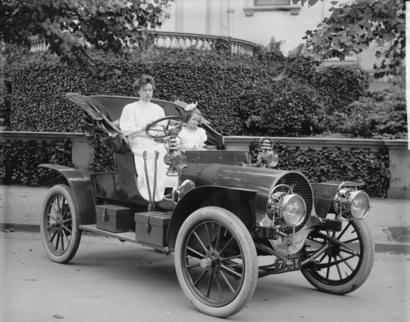
\includegraphics[width=\linewidth]{img/sample-franklin}
  \caption{1907 Franklin Model D roadster. Photograph by Harris \& Ewing, Inc. [Public domain], via Wikimedia Commons. (\url{https://goo.gl/VLCRBB}).}
  \Description{The 1907 Franklin Model D roadster.}
\end{figure}

Your figures should contain a caption which describes the figure to the reader. Figure captions go below the figure. Your figures should {\bf also} include a description suitable for screen readers, to assist the visually-challenged to better understand your work.

Figure captions are placed {\it below} the figure.

\subsection{The ``Teaser Figure''}

A ``teaser figure'' is an image, or set of images in one figure, that are placed after all author and affiliation information, and before the body of the article, spanning the page. If you wish to have such a figure in your article, place the command immediately before the \verb|\maketitle| command:
\begin{verbatim}
  \begin{teaserfigure}
    \includegraphics[width=\textwidth]{sampleteaser}
    \caption{figure caption}
    \Description{figure description}
  \end{teaserfigure}
\end{verbatim}

\section{Citations and Bibliographies}

The use of \BibTeX\ for the preparation and formatting of one's references is strongly recommended. Authors' names should be complete --- use full first names (``Donald E. Knuth'') not initials (``D. E. Knuth'') --- and the salient identifying features of a reference should be included: title, year, volume, number, pages, article DOI, etc. 

The bibliography is included in your source document with these two commands, placed just before the \verb|\end{document}| command:
\begin{verbatim}
  \bibliographystyle{ACM-Reference-Format}
  \bibliography{bibfile}
\end{verbatim}
where ``\verb|bibfile|'' is the name, without the ``\verb|.bib|'' suffix, of the \BibTeX\ file.

Citations and references are numbered by default. A small number of ACM publications have citations and references formatted in the ``author year'' style; for these exceptions, please include this command in the {\bf preamble} (before ``\verb|\begin{document}|'') of your \LaTeX\ source: 
\begin{verbatim}
  \citestyle{acmauthoryear}
\end{verbatim}

Some examples.  A paginated journal article \cite{Abril07}, an enumerated journal article \cite{Cohen07}, a reference to an entire issue \cite{JCohen96}, a monograph (whole book) \cite{Kosiur01}, a monograph/whole book in a series (see 2a in spec. document)
\cite{Harel79}, a divisible-book such as an anthology or compilation \cite{Editor00} followed by the same example, however we only output the series if the volume number is given \cite{Editor00a} (so Editor00a's series should NOT be present since it has no vol. no.),
a chapter in a divisible book \cite{Spector90}, a chapter in a divisible book in a series \cite{Douglass98}, a multi-volume work as book \cite{Knuth97}, an article in a proceedings (of a conference, symposium, workshop for example) (paginated proceedings article) \cite{Andler79}, a proceedings article with all possible elements \cite{Smith10}, an example of an enumerated proceedings article \cite{VanGundy07}, an informally published work \cite{Harel78}, a doctoral dissertation \cite{Clarkson85}, a master's thesis: \cite{anisi03}, an online document / world wide web resource \cite{Thornburg01, Ablamowicz07, Poker06}, a video game (Case 1) \cite{Obama08} and (Case 2) \cite{Novak03} and \cite{Lee05} and (Case 3) a patent \cite{JoeScientist001}, work accepted for publication \cite{rous08}, 'YYYYb'-test for prolific author \cite{SaeediMEJ10} and \cite{SaeediJETC10}. Other cites might contain 'duplicate' DOI and URLs (some SIAM articles) \cite{Kirschmer:2010:AEI:1958016.1958018}. Boris / Barbara Beeton: multi-volume works as books \cite{MR781536} and \cite{MR781537}. A couple of citations with DOIs: \cite{2004:ITE:1009386.1010128,Kirschmer:2010:AEI:1958016.1958018}. Online citations: \cite{TUGInstmem, Thornburg01, CTANacmart}.

\section{Acknowledgments}

Identification of funding sources and other support, and thanks to individuals and groups that assisted in the research and the preparation of the work should be included in an acknowledgment section, which is placed just before the reference section in your document. 

This section has a special environment:
\begin{verbatim}
  \begin{acks}
  ...
  \end{acks}
\end{verbatim}
so that the information contained therein can be more easily collected during the article metadata extraction phase, and to ensure consistency in the spelling of the section heading. 

Authors should not prepare this section as a numbered or unnumbered {\verb|\section|}; please use the ``{\verb|acks|}'' environment.

\section{Appendices}

If your work needs an appendix, add it before the ``\verb|\end{document}|'' command at the conclusion of your source document. 

Start the appendix with the ``\verb|appendix|'' command:
\begin{verbatim}
  \appendix
\end{verbatim}
and note that in the appendix, sections are lettered, not numbered. This document has two appendices, demonstrating the section and subsection identification method.

\section{SIGCHI Extended Abstracts}

The ``\verb|sigchi-a|'' template style (available only in \LaTeX\ and not in Word) produces a landscape-orientation formatted article, with a wide left margin. Three environments are available for use with the ``\verb|sigchi-a|'' template style, and produce formatted output in the margin:
\begin{itemize}
\item {\verb|sidebar|}:  Place formatted text in the margin.
\item {\verb|marginfigure|}: Place a figure in the margin.
\item {\verb|margintable|}: Place a table in the margin.
\end{itemize}

%
% The acknowledgments section is defined using the "acks" environment (and NOT an unnumbered section). This ensures
% the proper identification of the section in the article metadata, and the consistent spelling of the heading.
\begin{acks}
To Robert, for the bagels and explaining CMYK and color spaces.
\end{acks}

%
% The next two lines define the bibliography style to be used, and the bibliography file.
\bibliographystyle{ACM-Reference-Format}
\bibliography{sample-base}

% 
% If your work has an appendix, this is the place to put it.
\appendix

\section{Research Methods}

\subsection{Part One}

Lorem ipsum dolor sit amet, consectetur adipiscing elit. Morbi malesuada, quam in pulvinar varius, metus nunc fermentum urna, id sollicitudin purus odio sit amet enim. Aliquam ullamcorper eu ipsum vel mollis. Curabitur quis dictum nisl. Phasellus vel semper risus, et lacinia dolor. Integer ultricies commodo sem nec semper. 

\subsection{Part Two}

Etiam commodo feugiat nisl pulvinar pellentesque. Etiam auctor sodales ligula, non varius nibh pulvinar semper. Suspendisse nec lectus non ipsum convallis congue hendrerit vitae sapien. Donec at laoreet eros. Vivamus non purus placerat, scelerisque diam eu, cursus ante. Etiam aliquam tortor auctor efficitur mattis. 

\section{Online Resources}

Nam id fermentum dui. Suspendisse sagittis tortor a nulla mollis, in pulvinar ex pretium. Sed interdum orci quis metus euismod, et sagittis enim maximus. Vestibulum gravida massa ut felis suscipit congue. Quisque mattis elit a risus ultrices commodo venenatis eget dui. Etiam sagittis eleifend elementum. 

Nam interdum magna at lectus dignissim, ac dignissim lorem rhoncus. Maecenas eu arcu ac neque placerat aliquam. Nunc pulvinar massa et mattis lacinia.

\end{document}
